\section{Blockchain}
Event ticketing companies already issue event tickets digitally. The question arises why it makes sense to use a BC where transactions are slow, expensive and for many users difficult to interact with. The following points explain the benefits of tokenized tickets on a data store which can be accessed by anyone. 

\begin{itemize}
	\item Since the tickets are stored on a public database, anybody can verify whether a ticket is real without the need of a trusted third party. Tickets cannot be counterfeit and sold to multiple parties. 
	\item Less intermediaries such as payment processors are needed because digital currencies are available in the BC ecosystem. 
	\item Tokenized tickets on an open ledger enable the interoperability between different products and application. Similar to other standards emerging in the BC ecosystem such as described in Section \ref{subsubsection:token-interfaces}, it allows different applications to plug into the system and benefit from network effects. As an example for such a network effect, not every event platform has to provide its own identity verification process for personalized tickets if the proofs of the identities are stored on a public ledger. This allows another event organizer to issue personalized tickets without the need of verifying all guests again.
	\item The decoupling of the data layer (e.g. BC) from the user interaction layer (e.g. GUI) naturally adds competition in the respective layer and yields to better products overall. Throughout this report the \textit{primary market} is defined as the point of sale and the initial distribution of the tickets. The secondary market or aftermarket is defined as the the resell process between guests. Comparing such an approach with today's landscape, one can think of having one shared database among companies such as Starticket\footnote{\url{https://www.starticket.ch/en}} and Ticketcorner\footnote{\url{https://www.ticketcorner.ch}} (primary market), eBay\footnote{\url{https://www.ebay.com}} and Ricardo\footnote{\url{https://www.ricardo.ch}} (secondary market). A reward mechanism built into an open system incentives primary markets as well as secondary markets to participate. 
	\item The end user must only check on his favourite ticketing platform if tickets are available since all platforms connect to the same ledger.
	\item Stakeholders such as affiliates and frontend application providers benefit from guaranteed and instant payouts since their reward is recorded in the SC. 
\end{itemize}

\begin{figure}[H]
    \centering
    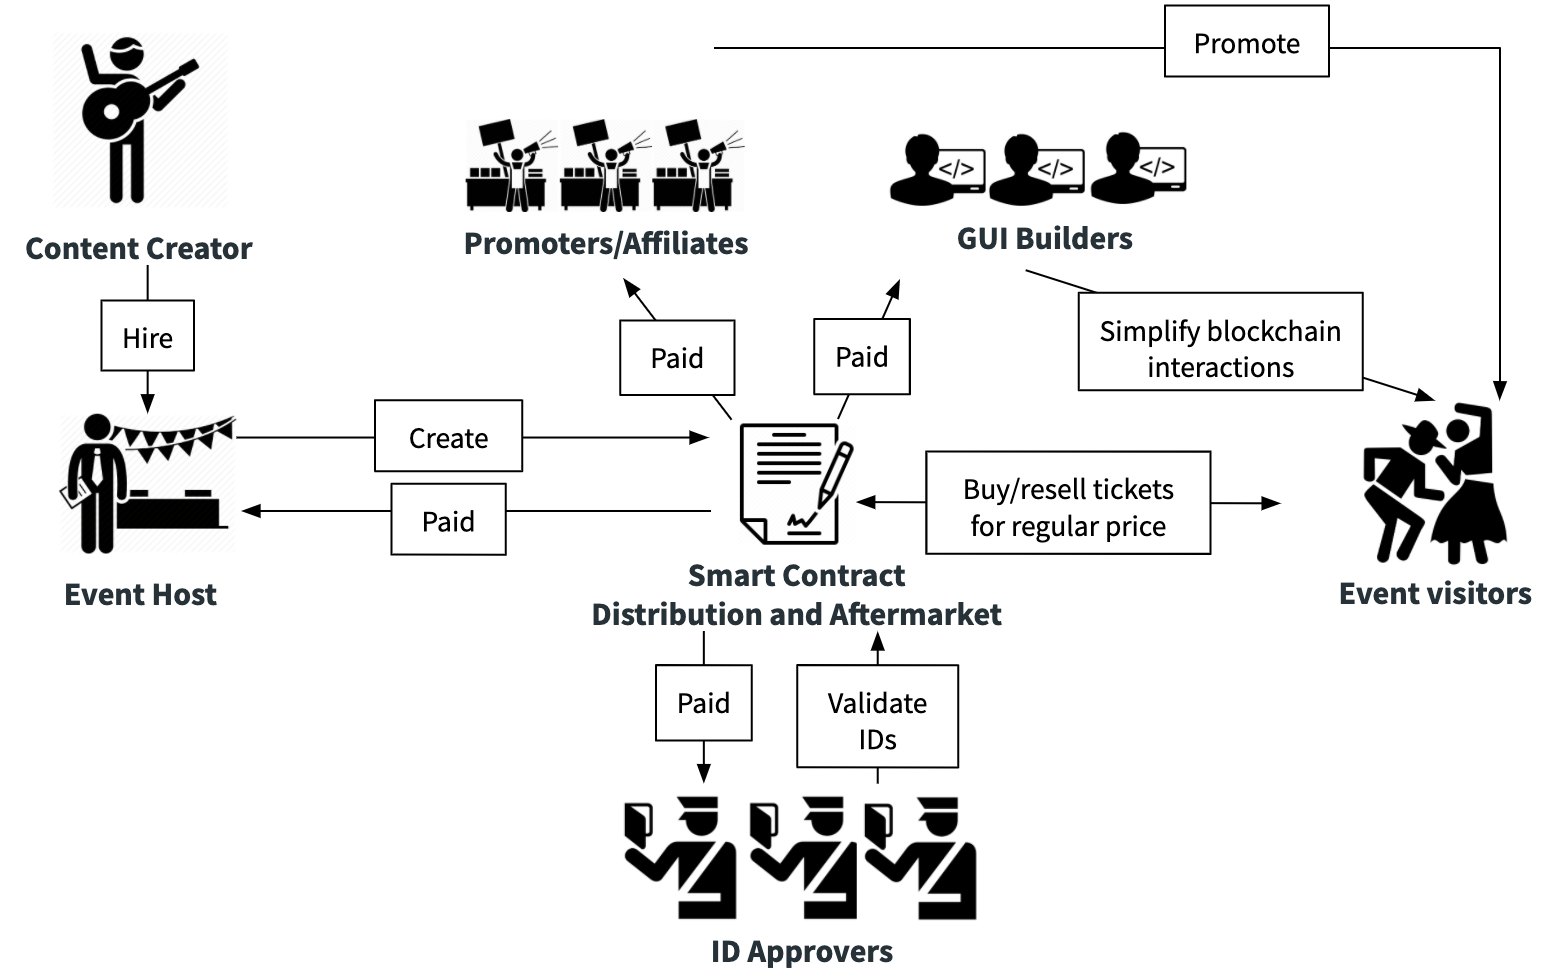
\includegraphics[width=16cm]{figures/dlt-based-landscape.png}
    \caption{DLT-based architecture}
    \label{fig:dlt-based-landscape1}
\end{figure}
